\subsection{Segment chest XRay(s) into multiple classes}
\label{sec:warmup6}

    In \cref{sec:warmup5}, we predicted only one mask, that is of lungs. In this exercise, we have to segment an xray into $4$ classes; lungs, heart, body and background. As the problem is similar to previous, we can utilize the same model as shown in \cref{fig:unet_lung} but with small modifications. 

\subsubsection{Dataset}
    The provided dataset have $200$ training x-ray images and $47$ testing images. As there was no validtion set, I have randomly splitted the training dataset into validation and training set in ration 1:9 respictively. Validation set is important as it allows one to verify model performance on hold-out set. The images in the datset are of size $256 \times 256$. The mask images are grayscale image of same size ($256 \times 256$) and have $4$ unique pixel values ($255$:lungs, $170$:body, $85$:heart, $0$:background). 

    The masks which are single channel image, have been converted to 4 channel image where each channel have information of a single mask.
    

\subsubsection{Training}
 
    As we have to geenrate $4$ masks, a small modification in model described in \cref{fig:unet_lung} has to be done before we can start the training. Instead of generating a single channel mask as output, we have to generate $4$ channel masks, Thus, the output channel needs to be changed from $1$ to $4$. After this modification the model is trained for 10 epochs using Adam optimizer with binary cross-entropy loss and learning rate of $10^{-2}$. \Cref{fig:organs-segmentation-learning-curve} shows the validation and training losses for each epochs. 

    \begin{figure}[htbp]
        \centering
        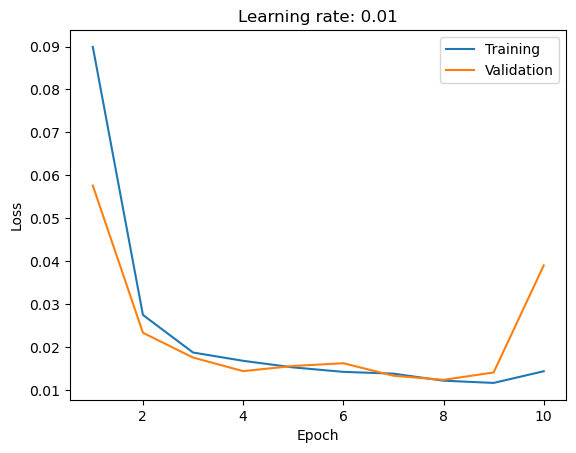
\includegraphics[width=\linewidth]{../plots/segmentation2/learning.png}
        \caption{Learning curve of Modified UNet \cref{fig:unet_lung} for generating $4$ masks.}
        \label{fig:organs-segmentation-learning-curve}
    \end{figure}


    \subsubsection{Result}
    
    After training the model, the model was tested on the provided test set and IoU, DICE scores reported in \cref{tab:organ-segmentation-result}. We can also observe the predicted masks in \cref{fig:organs-segmentation-result1} and \cref{fig:organs-segmentation-result2} and can say that model is able to generate near to accurate masks.

    \begin{table}
        \centering
        \begin{tabular}{cccccc}
          \toprule
            & Background & Heart & Body & Lungs & Avg. \\
          \midrule
           IoU & 0.623 & 0.734 & 0.884 & 0.881 & 0.781 \\
           DICE & 0.737 & 0.840 & 0.937 & 0.936 & 0.863 \\
          \bottomrule
        \end{tabular}
        \caption{Organs segmentation result}
        \label{tab:organ-segmentation-result}
      \end{table}

 
    \begin{figure*}[htbp]
        \centering
        \begin{subfigure}{0.8\linewidth}
            \centering
            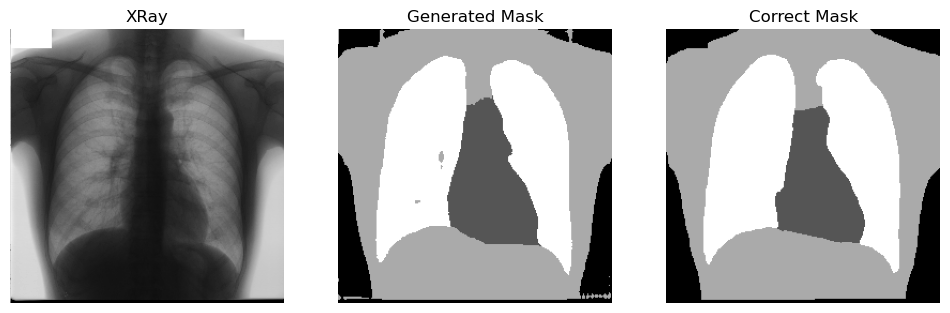
\includegraphics[width=\linewidth]{../plots/segmentation2/result1.png}
            \caption{Predicted masks, and target masks of a test XRay}
            \label{fig:organs-segmentation-result1}
        \end{subfigure}
        \begin{subfigure}{\linewidth}
            \centering
            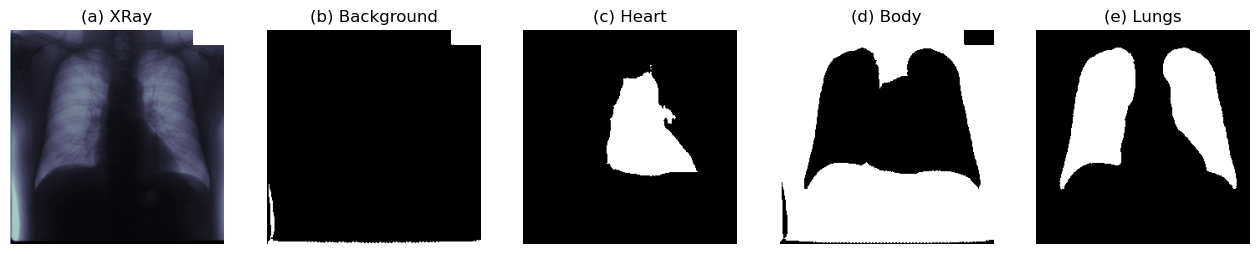
\includegraphics[width=\linewidth]{../plots/segmentation2/result2.png}
            \caption{Individual predicted masks of a test XRay }
            \label{fig:organs-segmentation-result2}
        \end{subfigure}
    \end{figure*}